% ===============================================================
% 		 		I N T R O D U C T I O N    G É N É R A L E
% ===============================================================
\chapter{Introduction générale}
\vspace{20pt}
\begin{center} {\scshape\bfseries sommaire} \end{center}
\startcontents[chapters]

\smash{\rule{\textwidth}{.4pt}}
\printcontents[chapters]{l}{1}{\setcounter{tocdepth}{3}}
\smash{\rule{\textwidth}{.4pt}}

\vspace{20pt}

\mylettrine{A}{l} Qâdî 'Iyâd Ibn Mûsâ Al Yahsûbî (1083-1149) (476 - 544 de l'hégire) était un cadi (juge) d'origine andalouse, affilié à l'école juridique malikite et à l'école théologique ash'arite. Il est un des sept saints de Marrakech.
Al Qâdî 'Iyâd appartenait à un clan arabe historique d'origine yéménite remontant à l'Imâm Mâlik Ibn Anas, qui s'était fixé à Baza, en Andalousie. À la suite de la conquête du Maghreb occidental par les Omeyyades de Cordoue, Ibn Abi 'Amr, soucieux de contrôler la route de l'or, fit installer de nombreux Andalous au Maghreb. C'est dans ce cont1exte que le père du Qâdî 'Iyâd s'installa à Ceuta.
Après avoir séjourné à Al-Andalus, Iyâd quitta Fès pour Kairouan.
Ayant terminé ses études, il partit en Andalousie pour y suivre l'enseignement de plusieurs maîtres avant de retourner à Ceuta en 1121. Après avoir occupé divers postes à Grenade, il devint en 1145 cadi de l'école malékite de Ceuta. Il est l'auteur de plusieurs ouvrages sur l'islam, dont Ash-Shifa bi ta'rif huquq al-Mustafa. Il a joué un grand rôle politique à la tête du mouvement de résistance anti-almohade. Après la victoire de son mouvement, il est contraint à l'exil à Marrakech, où il meurt en 1149.

\section{Chapitre 1}





\subsection{Formules mathématiques latex}

\begin{align*}
  f(x) &= x^2\\
  g(x) &= \frac{1}{x}\\
  F(x) &= \int^a_b \frac{1}{3}x^3
\end{align*}


\subsection{Sous section 2}

La figure \ref{fig:linear_regression} montre un exemple d'application de la régression linéaire.

\begin{figure}[H]
	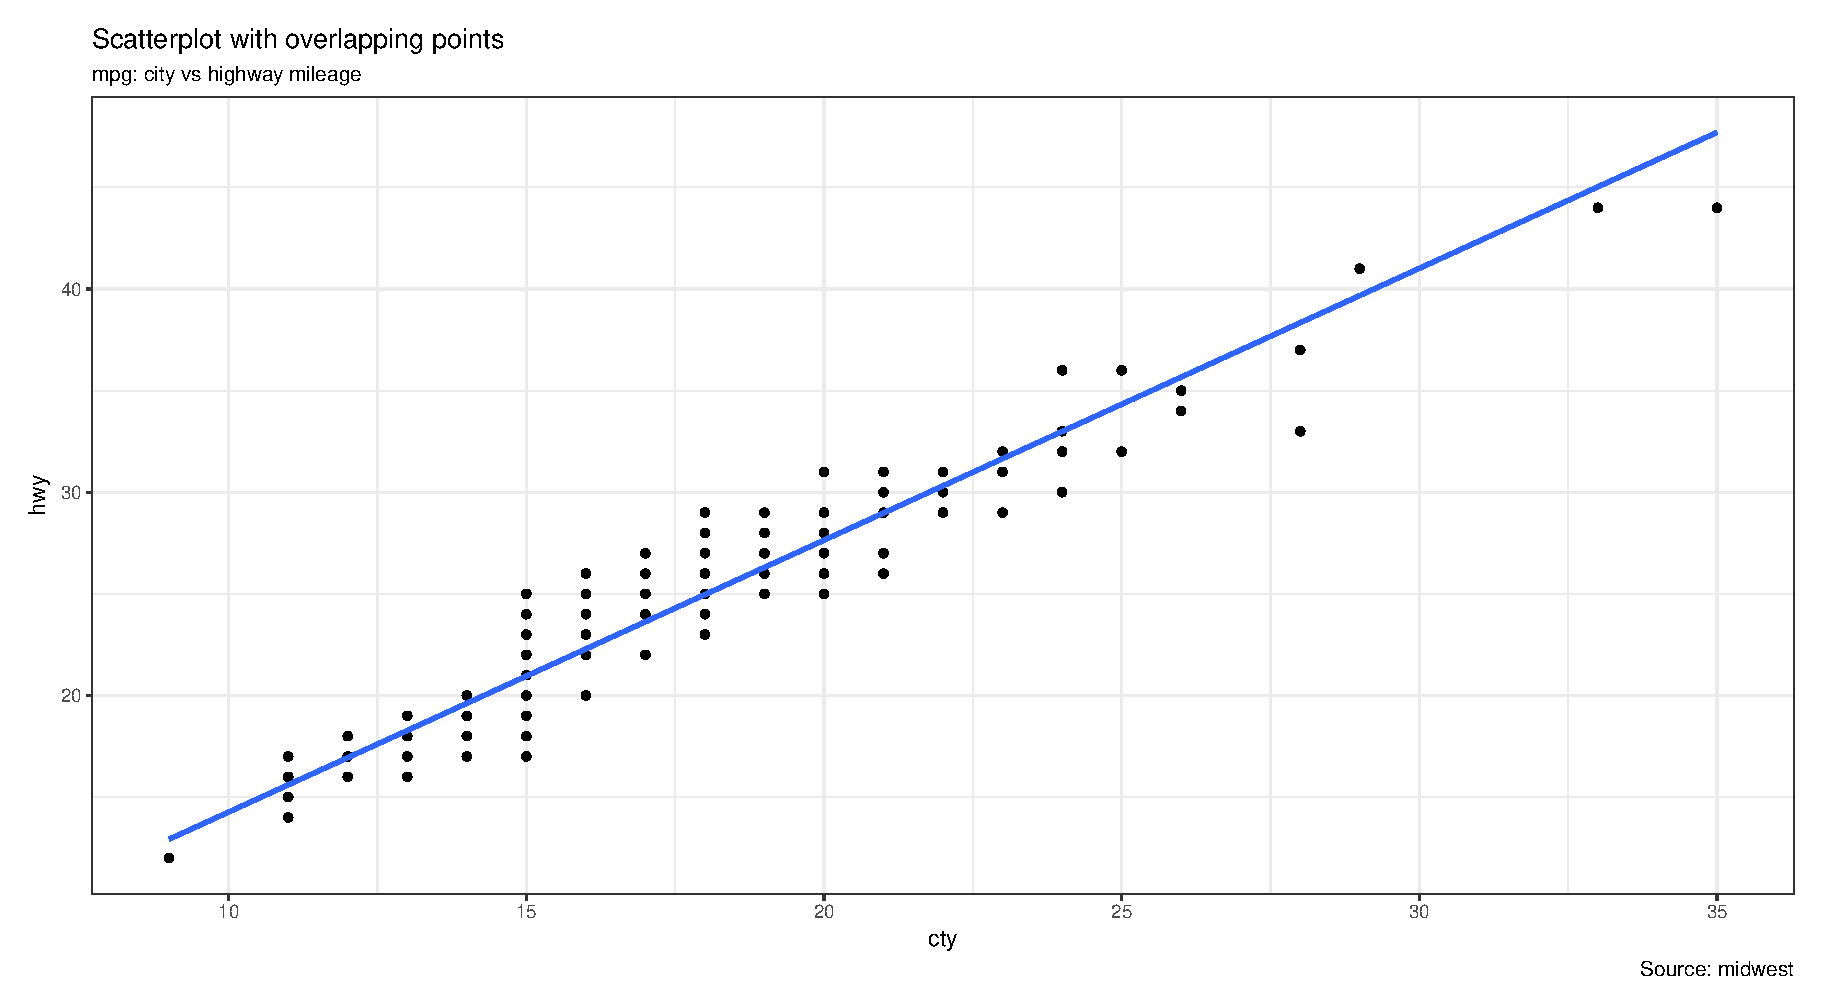
\includegraphics[width=1.0\textwidth,height=0.4\textheight]{Figures/chap1/linear_regression.eps}
	\caption{régression linéaire.}
	\label{fig:linear_regression} 
\end{figure}


\section{Section 2}

La figure \ref{fig:logistic_regression} montre un exemple de classification linéaire.

\begin{figure}[H]
	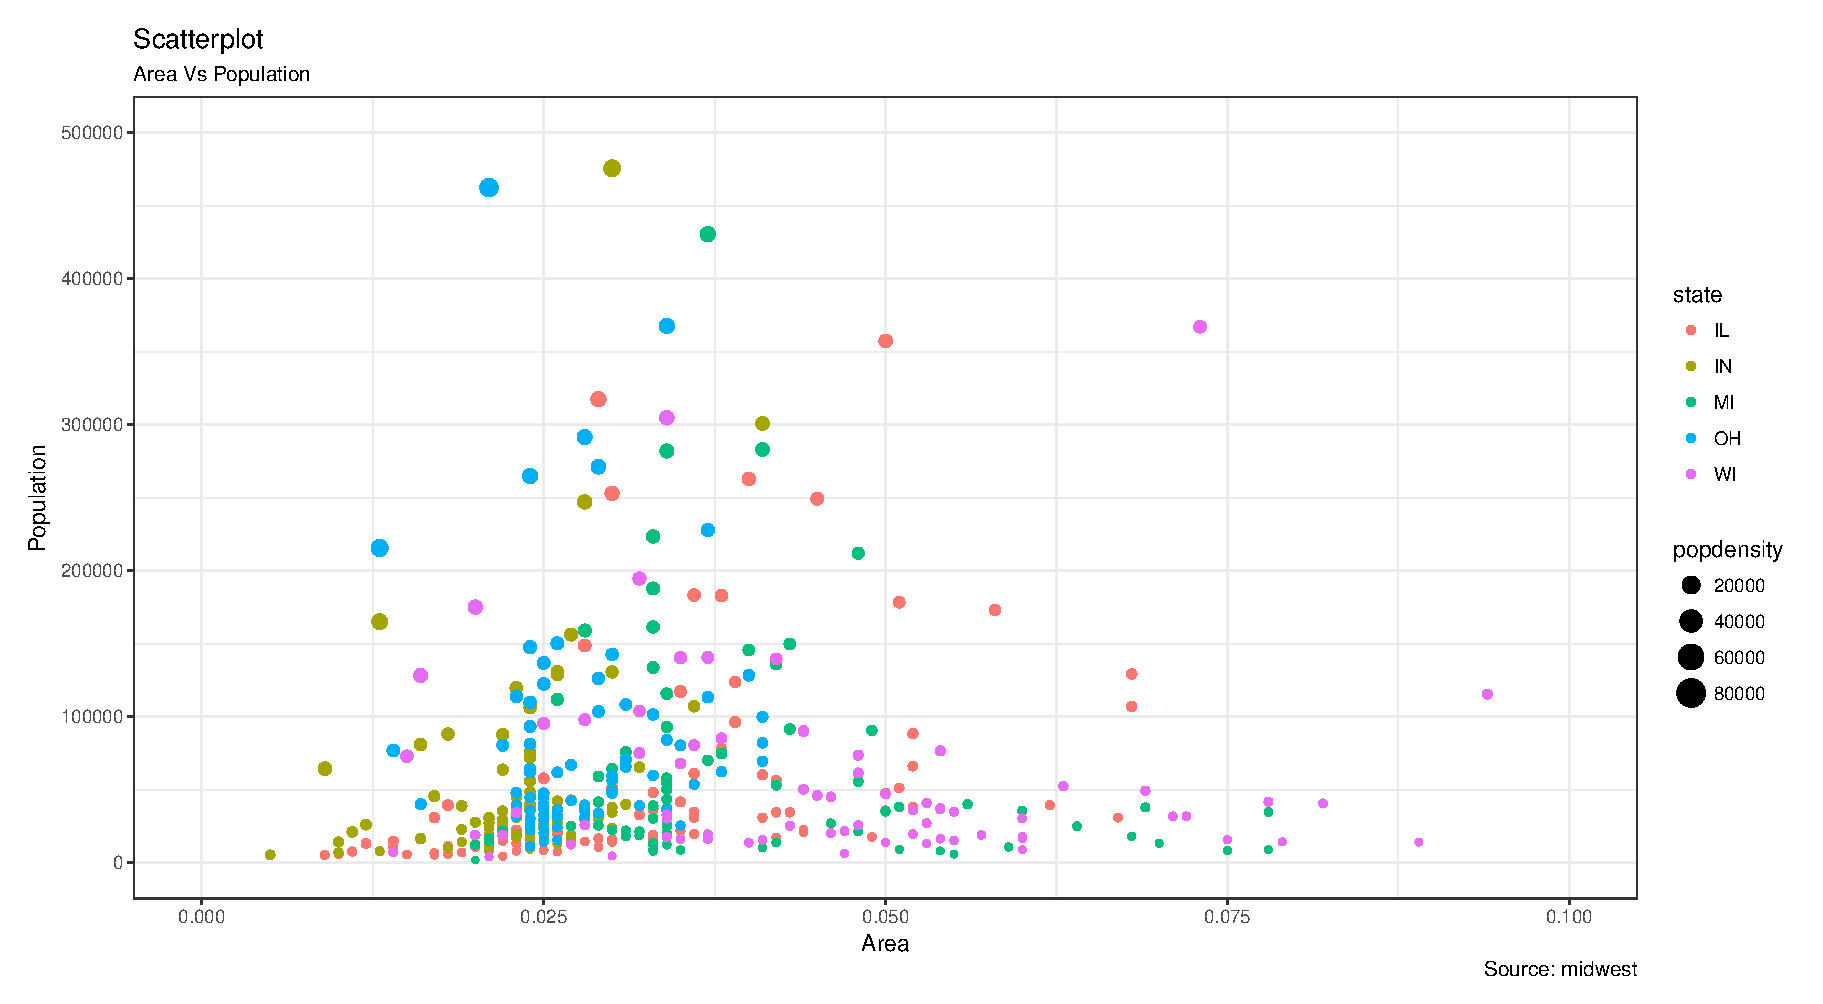
\includegraphics[width=1.0\textwidth,height=0.4\textheight]{Figures/chap1/logistic_regression.eps}
	\caption{Classification linéaire.}
	\label{fig:logistic_regression} 
\end{figure}

\subsection{Sous section 1}
\subsection{Sous section 2}

\section{Section 3}

\subsection{Sous section 1}
\subsection{Sous section 2}
\subsection{Sous section 3}
